\documentclass[12pt,openright,twoside,a4paper,english]{abntex2}
\selectlanguage{english}
\usepackage[utf8]{inputenc}
\usepackage{graphicx}
\usepackage{capa-epusp-abntex2/capa-epusp-abntex2}  % ver https://github.com/brunocfp/capa-epusp-abntex2/blob/master/README.md
% Folha de estilo: http://www.poli.usp.br/bibliotecas/servicos/publicacoes-online.html
% http://pro.poli.usp.br/wp-content/uploads/2012/04/NGTF2017.pdf
% http://www.poli.usp.br/images/stories/media/download/bibliotecas/DiretrizesTesesDissertacoes.pdf
% http://sites.poli.usp.br/d/pme2599/Documentos/Diretrizes%20de%20elabora%C3%A7%C3%A3o%20do%20trabalho%20final.pdf
\usepackage[alf]{abntex2cite}	% Citações padrão ABNT
\usepackage{float}
\graphicspath{{./images/}}

\author{TIAGO KOJI CASTRO SHIBATA\\
HENRIQUE CASSIANO SOUZA BARROS\\
VICTORIA AKINA TANAKA}
\orientador{BRUNO DE CARVALHO ALBERTINI}
\areaconcentracao{Computer Engineering}
\preambulo{Monograph of the capstone project of the Computer Engineering bachelor - Escola Politécnica da Universidade de São Paulo}
\title{ColorMotion: Automatic video colorization}
\date{São Paulo\\(November 2018)}

\begin{document}
\begin{otherlanguage}{english}

\imprimircapa
\imprimirfalsafolhaderosto
\imprimirfolhaderosto

\begin{epigrafe}
\begin{flushright}
\vspace*{\fill}

\textit{``It is the supreme art of the teacher to awaken joy in creative expression and knowledge``}\\
(Albert Einstein)
\par\end{flushright}\end{epigrafe}

\begin{resumo}
Given a grayscale video, this monograph proposes a method for colorization using convolutional neural networks in an encoder-decoder architecture. Unlike current image colorization models which, when applied frame by frame, create inconsistencies between frames, this model maintains state in the encoded features and learns to colorize while maintaining the colors of regions that existed on previous frames. Dense optical flow is used to track movement and propagate colors between frames. The method is user-guided in the sense that an user can input pixel colors as additional information, biasing the algorithm at multimodal color choices. Training was done on large scale datasets taken from open source videos and the ImageNet dataset, which was artificially augmented to generate frame sequences with motion.
\vspace{\onelineskip}

\noindent
\textbf{Keywords}: CNN. Colorization. Video. Restoration. Encoder-decoder.
\end{resumo}

%TODO listas de gráficos, tabelas, abreviaturas e siglas, símbolos
%DNN - Deep Neural Network
%CNN - COnvolutional Neural Network
%MSE - Mean Squared Error

\cleardoublepage

\tableofcontents

\maketitle

\chapter{Introduction}
In this monograph, we propose a method for automatic video colorization, using a machine learning-based approach.

Previous work \cite{colorful} has used CNNs trained on large-scale datasets to colorize pictures successfully. However, when applied frame by frame on videos, the predictions have inconsistencies between frames, since no state is maintained between frames and different colors are predicted on the same object after small changes in the input grayscale image.

Since the colorization problem is multimodal, that is, multiple colors are plausible colorizations for a single object, the proposed model can also be user-guided. The algorithm can take input colors for a given object (e.g. the user can choose a t-shirt's color to be red) and will colorize the object and propagate it to following frames.

\section{Motivation} \label{sec:Motivation}
The problem of colorization in the field of machine learning is one of major interest. It is not a solved problem and poses challenges unlike others, since its solutions are multimodal (the same object has multiple plausible colorizations). Previous research showed that generating believable colorizations is hard, since commonly used objective functions will infer conservatory colors in multimodal regions to minimize the loss, generating images with too low saturation to be convincing \cite{colorful}.

Our work automates a manual, boring and expensive process: professional picture and video restoration services require expertise and lots of manual inputs from a trained professional. Restoration of videos costs upwards of thousands of dollars per minute: on a quote done with a prominent company in the sector, the restoration of a 9 minute video using their lower quality tier would cost USD 23000,00.

\section{Model overview}

We take colorization of videos to be an extension of the colorization of images. We propose the use of state-of-the-art machine learning algorithms to colorize videos, prioritizing methods to maintain consistency of colors between frames in a scene whilst correctly colorizing new objects in a frame and detecting frames associated with a new scene. Our base model architecture is heavily based on previous image colorization work, with added state and an intermediate dense optical flow step. The intermediate dense optical flow step using the Lucas-Kanade method makes the model non-differentiable and, thus, not an end to end trainable CNN; however, we achieve good results training the encoder and decoder separately.

\section{Evaluation}
Results are trained on large scale data using open source videos, personal videos collected by the authors, and ImageNet images augmented to have artificial motion. %TODO insert loss imformation
The results are then tested on people: Volunteers were asked to rate scenes as original or computer colorized, so we can have a metric on how believable the colorization is.

\section{Justification}
As stated in section \ref{sec:Motivation}, the traditional process of coloring images involve manual inputs from the user and use of advanced professional editing tools.
%TODO: citation needed, probably something about restoring pictures
The same can be said to the colorization of videos, with the added difficulty of maintaining consistency through frames. Some tools can help tracking the motion and colors between frames, but the initial input and challenges involving rapidly changing scenes add to the complexity of the process. These tools often are integrated with other editing software, such as the Mocha plugin \cite{mocha} and the SilhouetteFX Suite \cite{silhoutte}, being utilized as general purpose tools, mainly for color correction.
%TODO:citar como eles fazem o tracking?

\chapter{Related work}
Most of the previous works studied were concerned with the problem of coloring images. One traditional method to resolve this problem was inaugurated by Levin  \textit{et al.} \cite{Levin2004},
where colorization is achieved through quadratic cost-functions to determinate the color of neighbouring pixels, and the initial colors are given by scribbles input by the user. This type of approach has received improvements in following works \cite{Kumar2012},
%TODO: citar mais um trabalho pós-Levin
but the necessity of user-guidance has always represented a compromise in the process.

One method to simplify the scribble-based approach is the reference-approach, were a reference image is supplied rather than local colors. This method is explored by Kumar \textit{et al.} \cite{Kumar2012},
where pixels are grouped for both feature extraction and color classification, which in turn is resolved via a randomized decision forest. The reference-approach method is also employed in other problems in the image domain, such as style-transfer.
%TODO: citar o trabalho de transferência de estilo (relevante aqui imo)

The first fully-automated technique created was developed by Cheng \textit{et al.} \cite{Cheng2015},
where a DNN is employed with feature descriptors as the input layer and with UV channels as the output, for each pixel and in the YUV colorspace.

Most of the state-of-the-art algorithms applied today involve the use of Convolutional Neural Networks.
%TODO: citar CNNs (Larsson, Lizuka). Focar no colorful
The state-of-the-art work in the field applies methodologies such as described in Zhang \textit{et al.} \cite{colorful}

%TODO: talvez inlcuir Learning Large-Scale Automatic Image Colorization como referencia
%TODO: Importar nossos resumos do Mendeley

%1) Levantamento bibliográfico em bases de dados nacionais e internacionais, a
%partir de palavras-chave em português e inglês;

%2) Busca pelos textos completos dos trabalhos selecionados no levantamento;

%3) Leitura e fichamento (resumo analítico) dos trabalhos relevantes. É imprescindível anotar os dados dos documentos consultados, para posterior citação e referência;

%4) Cruzamento de informações e citações de modo a elencar um quadro de autores sobre o assunto, alinhados com o ponto de vista do pesquisador;

%5) Redação da revisão e citações, de acordo com o assunto e tópicos abordados.

%A learning-based approach for automatic image and video colorization

\chapter{Methodology}

We adopted four main phases of development: study and choice of existent machine learning algorithms; development of a dataset; specification of the initial neural network architecture; adaptation the architecture to improve model performance and add new features (such as the use of recurrent architectures to maintain state and the use of dense optical flow); and collection of metrics and user feedback based on A/B tests.

\section{Conceptual aspects} \label{sec:Concept}
Neural networks for colorization can be divided in two broad categories: those that require inputs from the user, and those that use a automated process. In both cases, the most modern approaches use Convolutional Neural Networks (CNN) to leverage different image characteristics, and use those patterns to identify and separate objects in the image and colorize them accordingly. Other approaches are possible, for example through the use of self organizing maps alongside neural networks as shown in Richart \textit{et al.} \cite{Richart_som_nn}; but for the purposes of this monograph we will focus in CNN-based algorithms.

Fully convolutional DNNs were used throughout this work to take advantage of its space invariance and local correlation between pixels in an image.

\section{Dataset}
\subsection{Colorspace}
As stated on Colorful %TODO: cite
and seen on related research, the L*a*b colorspace is most suitable for the colorization task. It's L* channel is the achromatic lightness quantity, which depends solely on the perceptually achromatic luminance. Thus, the perceptual lightness of a colorized image to a human observer appears most similar in lightness to a grayscale image when using the L*a*b* colorspace and maintaining the L* value. We use all network input images as a single channel L* image, and all color outputs are given in the a*b* colorspace.

\begin{figure}[!htb]
\centering
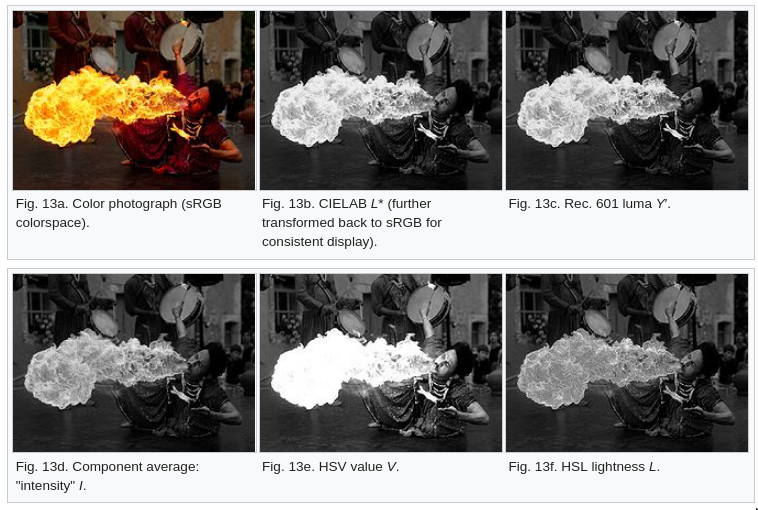
\includegraphics[width=\textwidth]{Colorspaces}
\caption{Source: https://en.wikipedia.org/wiki/HSL\_and\_HSV }
%TODO: adicionar como citação)
\label{hsl_hsv}
\end{figure}

\subsection{Processing of scenes from movies}

We wanted a dataset made of open source content, with permissive licenses. After some research, we decided to use the open source movies Tears of Steel and Valkaama as a starting point. %TODO adicionar citações dos filmes e links para páginas dos projetos

To split the movies into independent scenes, two strategies were employed. We created a program to compute the structural similarity index (SSIM) between each pair of frames and, whenever the SSIM was high, we assumed a new scene was starting. The SSIM is similar to the simpler, less robust mean squared error (MSE) metric, except it's more resistant to noise and compression artifacts.

We also ran a histogram analysis on the pixel values of each frame and discarded frames without enough variability. This strategy removed introduction frames, black frames from fading effects, final credits and other undesired frames whose content had very low variability.

After running a script with both algorithms, the result was almost perfect. A few scenes containing too fast movement (yielding a high SSIM) were cut into multiple scenes and had to be manually inspected and fixed. After filtering and splitting the scenes, the dataset had 142753 frames in 836 distinct scenes. This small dataset was used as a starting point.

The dataset structure was exported to files describing ranges of frames corresponding to each scene. This metadata was written in JSON format to make re-creation of the dataset easier in other machines. It's avaiable on https://github.com/ColorMotion/Dataset.  %TODO trocar por citacao

\section{Baseline model}

Our first, baseline model was created using a convolutional DNN. We borrowed the same architecture used in Colorful \cite{colorful}, except we reimplemented it in Keras. Our main goal with this model was to gain familiarity with the tooling we would use in the rest of the work.

The architecture implements an encoder-decoder architecture with skip connections. To enlarge the receptive field of convolutions with encoded features and empower the network to detect larger features, encoded features go through dilated convolutions.
%TODO falar mais da arquitetura?

\subsection{Objective function}

The objective function used in the baseline model is the mean squared error (MSE) since it'e easy to use. Related work \cite{colorful} shows that MSE is not a good objective function to create convincing colorizations, since it gives very conservative predictions in multimodal objects, creating undersaturated images. Other methods, such as regressing a color probability distribution function \cite{colorful}, would be more suitable, but are harder to implement and train.

\subsection{Environment}

We prepared an environment for training in the cloud. GPUs available in servers are more powerful than the ones we own and have more RAM to cope with large models. The chosen cloud provider was Paperspace %TODO cite https://www.paperspace.com/
due to its lower cost when compared to other providers.

A Docker container was created so we could prepare the environment and easily port it to other machines. The environment can be found at , %TODO cite https://github.com/ColorMotion/ColorMotion-docker
and contains NVIDIA CUDA libraries, Keras, TensorFlow, Python, and other project dependencies. The container is run with nvidia-docker, %TODO cite https://github.com/NVIDIA/nvidia-docker
a project that allows containers to access NVIDIA GPUs so that CUDA applications can be containerized.

Funcionou
implementação OK
Mostrar modelo do paper
indicar modelo anexo
Explicar Lambda

8000 (initial loss without pretrained weights)

mmtoir

transfer

retraining

%TODO inserir curvas de perda dos testes iniciais em teste/validação

After initial training, this dataset proved too small for the task in hand. In our methodology, we employed a network with a high number of parameters, which is very prone to overfitting. The network did overfit a lot in our initial tests, as can be seen by the loss MSE of 4.21 and validation MSE of 98.43.

\begin{figure}[!htb]
\centering
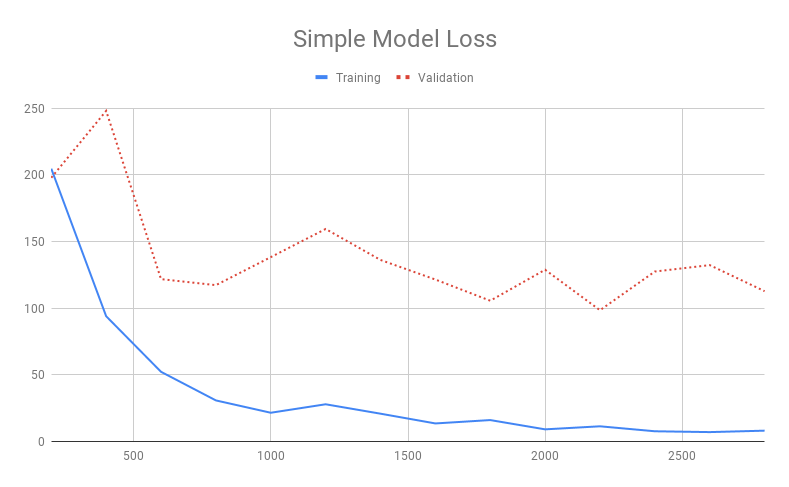
\includegraphics[width=\textwidth]{loss/Simple}
\caption{Simple model loss}
\label{simple_loss}
\end{figure}

Augmentation:

%TODO document Keras augmentation

The dataset was enlarged with videos from the free video repository Pixabay, under the Creative Commons licence, and from videos in the author's personal archives. The enlarged dataset has 591780 frames in 1629 distinct scenes. Data augmentation was also implemented during training to reduce the amount of overfitting to the training dataset. Augmentation was

Lastly, part of the ImageNet \cite{imagenet_cvpr09} dataset was downloaded from the URLs provided in the ImageNet website. The dataset has a variety of pictures belonging to one of thousands of "synonym sets". 1071981 images were used during training of the user guided colorization model.
%TODO document augmentation. TODO show reduced overfitting, show loss curves.

% \subsection{Choice of algorithm}
% Like stated on section \ref{sec:Concept}, the

\subsection{Algorithm adaptation}
%TODO: descrever arquitetura

%TODO: descrever interpolação de features encodadas p/ manter estado do frame

%TODO: descrever função de perda

%TODO strategy: incremental enhancements and retraining, document importing weights from other models, document performance optimizations

\subsection{Optimization}
After these initial results, we achieved a validation MSE loss of 38.43.
%TODO: atualizar quando resultado melhorar.
Our initial training strategy was to start with a deep, large model and use model pruning techniques to remove layers that don't affect the result and compress the model while achieving similar performance. To this end,
%TODO: documentar métodos usados de poda (layer removal e APoZ).

\section{Used technologies}
Keras, OpenCV, numpy

\section{System specifications}
%TODO specs, performance analisys
Using a GTX1080 consumer level card, streaming the frames one by one (without batching) leads to inference times of 32ms in the unoptimized, large, deep model. Batching multiple frames yields average performance of up to 28ms/frame.


%O modelo final obteve 32ms/quadro em uma placa de nível de consumidor (NVIDIA GTX1080) com batches unitários, possuia 34051138 parâmetros treináveis, e após serializado ocupava 390MB. Após otimização (remoção de camadas e pesos pouco influentes pelo método Average Percentage of Zeros - APoZ) e uso de batches de 8 frames, obtivemos o desempenho de 28ms/quadro, com 28879168 parâmetros treináveis, e 111MB. O modelo é aplicável em fluxos de vídeo em tempo real.

\chapter{Results}
\section{Comparison to competing methods}

%TODO

\section{User tests}
%TODO some images
In order to validate the results obtained by the network, we ran ten seconds videos previously unbeknownst to the network by it. These videos were in 256X256 resolution. 0.016\% of the original a*b* values were used as guidance. The results were then shown to volunteers, who randomly received a series of original or artificially colorized videos. For each video, they were asked to determine if it was original or colorized by a computer. The results of these tests can be shown in \ref{table:ABresults}.
%TODO: quantas pessoas?
\begin{table}[H]
\centering
\begin{tabular}{l|l|l|ll}
\cline{2-3}
                                    & \multicolumn{2}{l|}{\textbf{Chosen}} &                           &  \\ \cline{1-3}
\multicolumn{1}{|l|}{\textbf{Real}} & \textbf{No}      & \textbf{Yes}      &                           &  \\ \cline{1-4}
\multicolumn{1}{|l|}{\textbf{No}}   & 40.4             & 7.9               & \multicolumn{1}{l|}{48.3} &  \\ \cline{1-4}
\multicolumn{1}{|l|}{\textbf{Yes}}  & 6.7              & 44.9              & \multicolumn{1}{l|}{51.7} &  \\ \cline{1-4}
                                    & 47.2             & 52.8              &                           &  \\ \cline{2-3}
\end{tabular}
\label{table:ABresults}
\caption{Results obtained after the AB tests.}
\end{table}

We observed that in the videos colorized by the network, \(7.9/40.4 = 19.6\% \) of volunteers  believed that the colors shown in the clip were real. In another test, the volunteers were shown both versions side by side and were asked to identify the clip with the real colors. 12.9\% of the time, volunteers where fooled and chose the colorized version.

\chapter{Discussion of achieved results}
One of the main results observed in the tests was the efficiency of the network in reproducing external enviromnents, specially landscapes, wildlife and vegetation, and conversely difficulty in coloring internal environments, human crafted objects and some specific, less common objects. This can be attributed to the multimodal nature of human crafted objects and environments, which lead to conservative predictions by the network with a low a*b* value.  The ImageNet-based dataset might also be skewed, having few internal enviromnents with multiple objects in sight. Better data collection and another objective function could help mitigate these issues.
%TODO image of stuff going right and wrong in terms of vegetation vs inside

Improvements would also be likely if we used a neural network for dense optical flow estimation instead of the Lucas-Kanade method. An intermediate neural network for dense optical flow could be trained end-to-end with the rest of the network and possibly achieve better global results. Currently, there are a few options for fast optical flow estimation in deep learning, and our network would likely remain usable in real time.
%TODO: fotos de casos onde a cor mudou pelo opt flow
%TODO: citar redes de opt flow
%TODO: citar transf. de estilo Microsoft




\chapter{Conclusions}


%TODO \chapter{Future work}? Por enquanto colocando na discussao
%\chapter{TODO glossary}
\chapter{Appendix}

\begin{figure}[!htb]
\centering
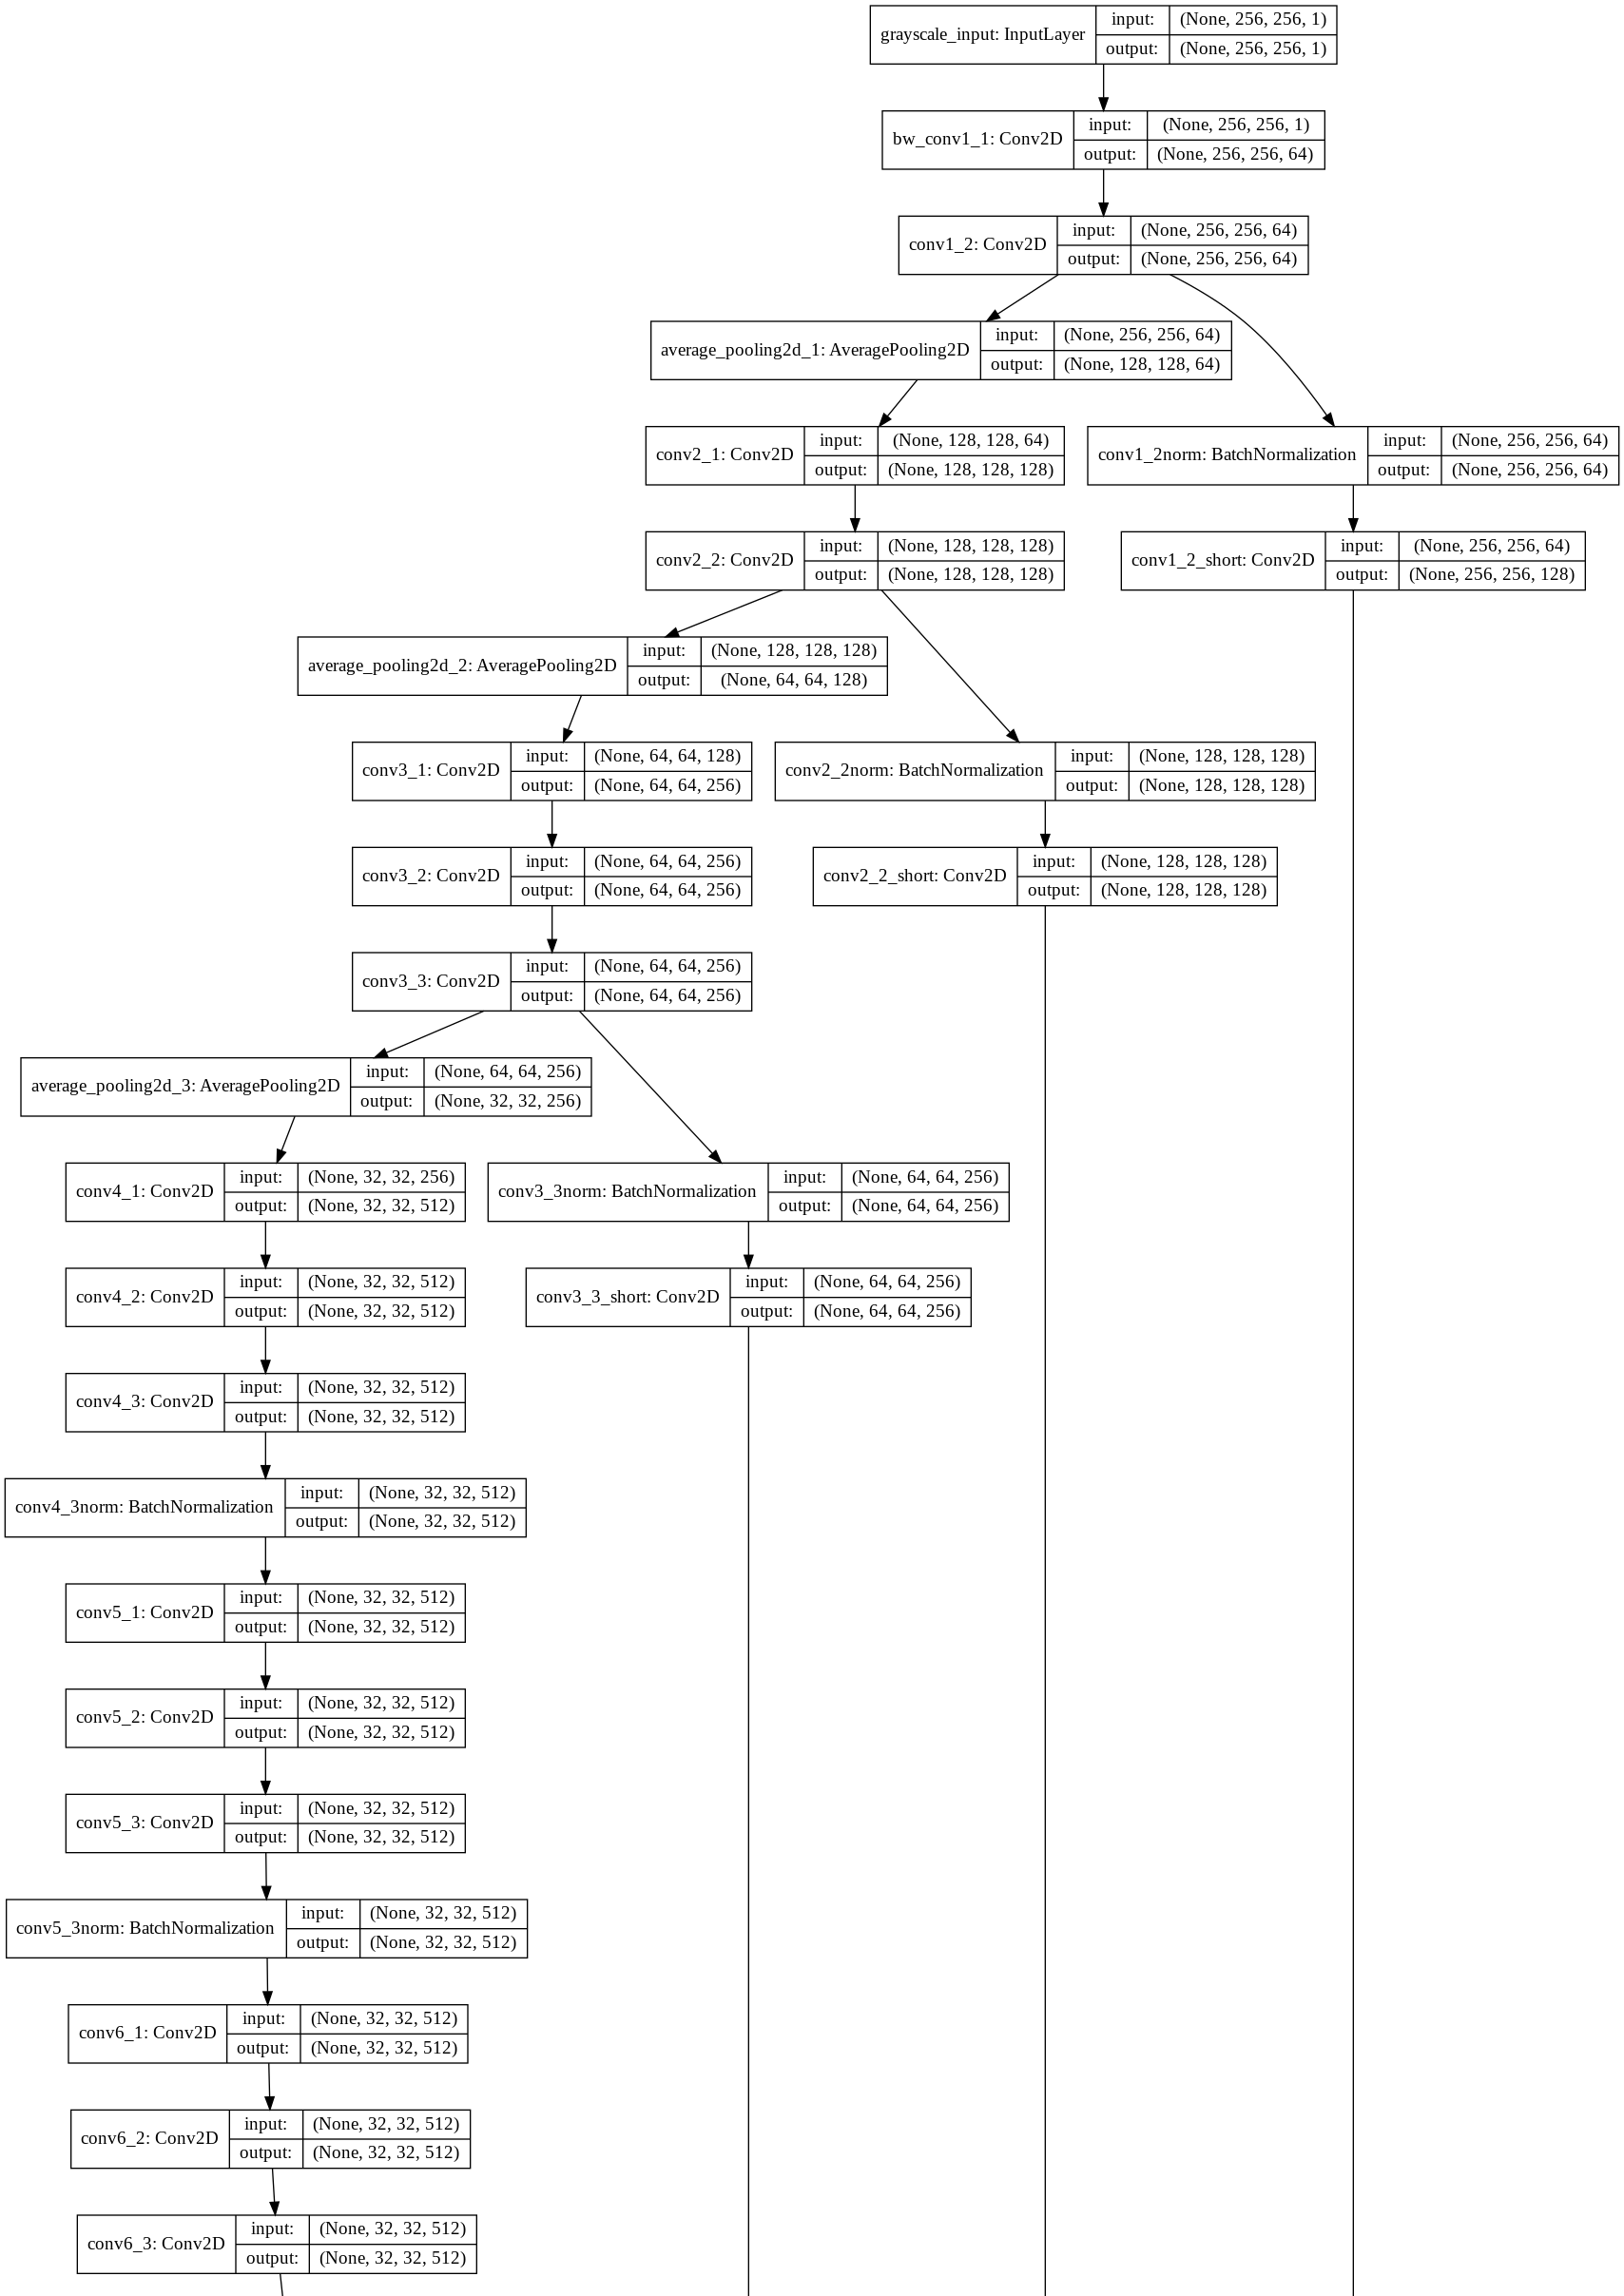
\includegraphics[height=\textheight]{model_plot/Simple1}
\caption{Simple model architecture expanded - Part 1}
\label{simple_plot}
\end{figure}

\begin{figure}[!htb]
\centering
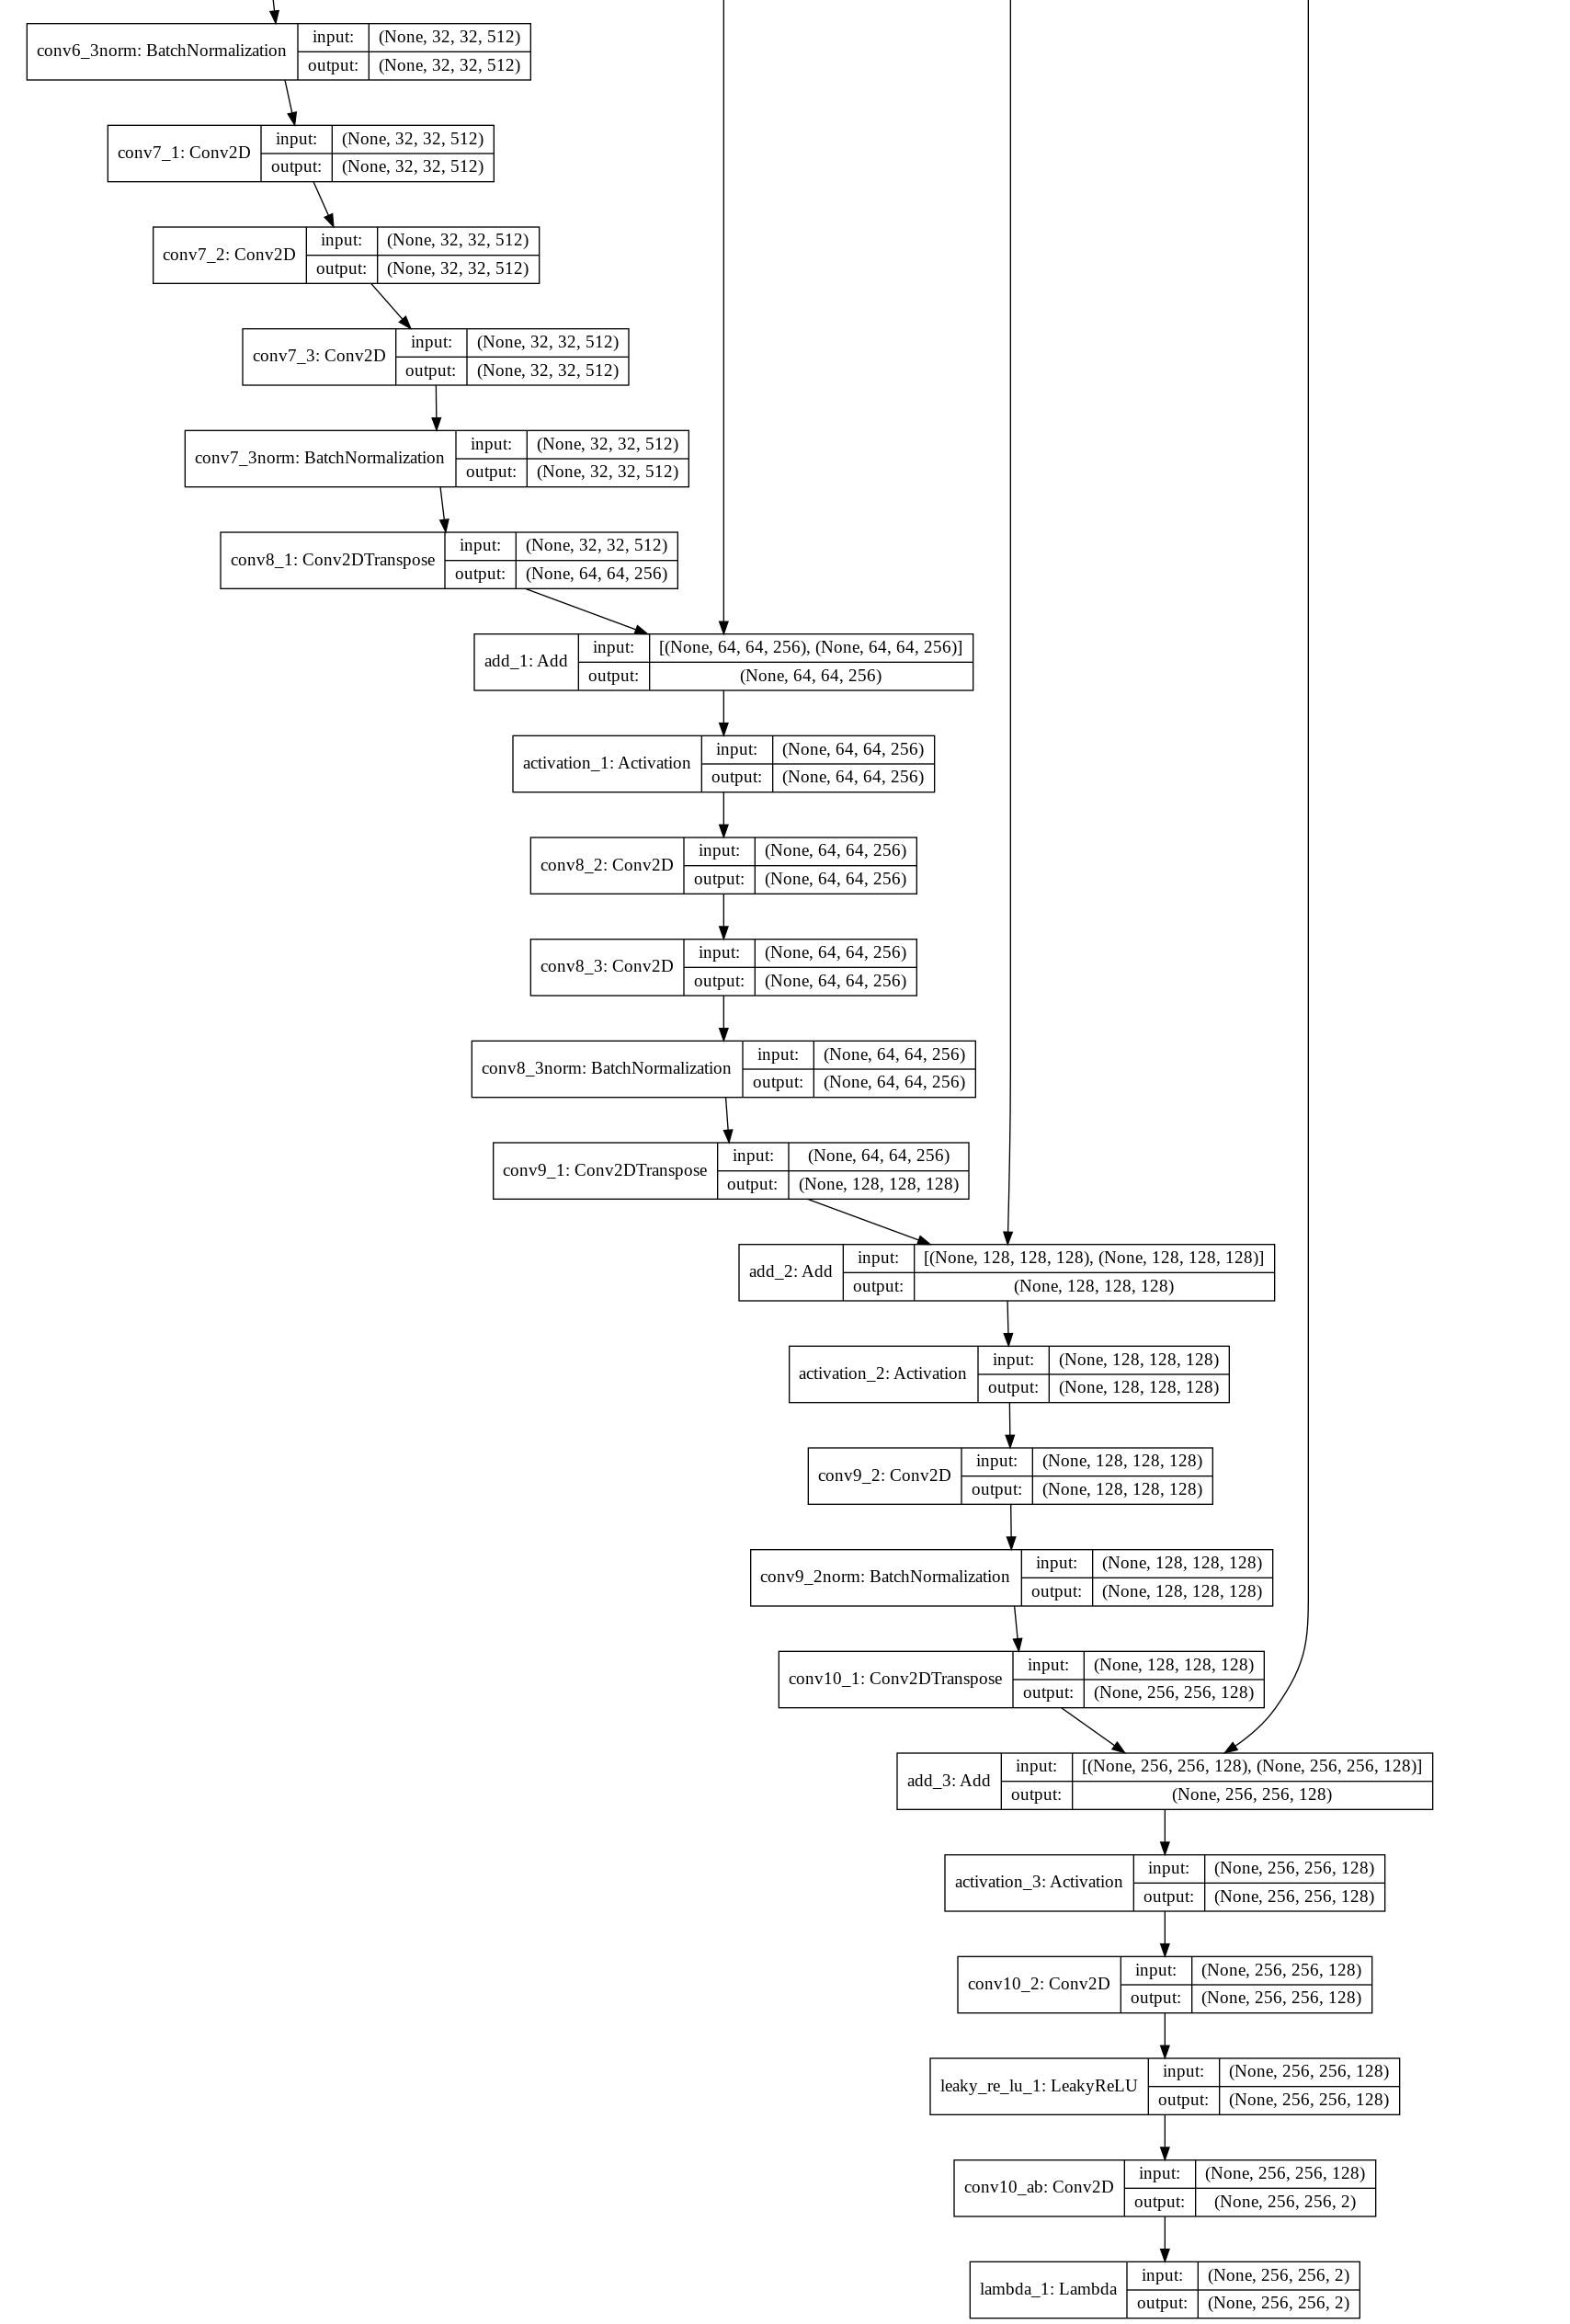
\includegraphics[height=\textheight]{model_plot/Simple2}
\caption{Simple model architecture expanded - Part 2}
\label{simple_plot}
\end{figure}

\bibliography{referencias.bib}
%\printbibliography

\end{otherlanguage}
\end{document}
